\documentclass[a4paper,11pt]{article}
    %% Used for changing geometry of the page
    %% Cover page text cannot overlay cover sketching/style 
    %% https://ctan.org/pkg/geometry?lang=en
\usepackage{geometry}
\geometry{
    top=30pt,
    left=40pt,
    right=40pt
}
    %% Changes language of some packages protocols
    %% e.g., when captioning images: Figure 1. -> Figura 1.
    %% https://ctan.org/pkg/babel?lang=en
\usepackage[portuguese]{babel}
    %% Used for special fonts
    %% Cannot be compiled with pdflatex
    %% https://ctan.org/pkg/fontspec?lang=en
\usepackage{fontspec}
    %% Arial FONT
    \setmainfont{Arial}
\usepackage{subfiles}
    %% More colors and color options
    %% https://ctan.org/pkg/xcolor?lang=en
    %% https://ctan.org/pkg/colortbl?lang=en
\usepackage{xcolor,colortbl}
    %% More tabular options, like dashed/dotted lines
    %% https://ctan.org/pkg/arydshln?lang=en
\usepackage{arydshln}
    %% List of acronyms
    %% https://ctan.org/pkg/nomencl?lang=en
\usepackage[intoc]{nomencl}
    %% Must be called to init nomencl environment  
    \makenomenclature
    %% More images options/settings
    %% https://ctan.org/pkg/graphicx?lang=en
\usepackage{graphics}
    %% Defining subdirectories to image path enviornment
    %% \graphicspath{{sub1}{sub2}...{subN}}
    \graphicspath{{images}}
    
    %% used to handle cross-referencing commands in LaTeX to produce hypertext links in the document
    %% https://ctan.org/pkg/hyperref?lang=en
\usepackage{hyperref}
    %% math environments
    %% https://ctan.org/pkg/amsmath?lang=en

    %% settings
    \hypersetup{
        colorlinks,
        citecolor=black,
        filecolor=black,
        linkcolor=black,
        urlcolor=black
    }

\usepackage[backend=bibtex, style=numeric-comp]{biblatex}
\addbibresource{biblio.bib}

\usepackage{amsmath}
    %% Defining backgrouns, used to make the cover
    %% https://ctan.org/pkg/background?lang=en
\usepackage[some]{background}
    %% Used to make drawings or complex graphics
    %% http://pgf.sourceforge.net/pgf_CVS.pdf
\usepackage{tikz}
    %% Tikz library to point operations ((x1,y1) + (x2,y2))
    \usetikzlibrary{calc}
\usepackage{lscape}
%% Defining sfdefault font and default font for document
\renewcommand{\familydefault}{\sfdefault}

\usepackage{float}

\usepackage{minted}
\setminted[java]{ %
    autogobble=true,          % Automatically remove common white space
    frame=lines,
    breaklines,
    framesep=2mm,
    fontsize=\footnotesize
}

\usepackage{multicol}

%% Costume made cover 
%% From there you can use \makecover command to build the cover
%% Blue cover color
\definecolor{titlepagecolor}{RGB}{54,95,145}

%==========================================================================
% COLORED BAR ON THE LEFT SIDE
%==========================================================================

\backgroundsetup{
    scale=1,
    angle=0,
    opacity=1,
    contents={
            \begin{tikzpicture}[remember picture,overlay]
                \path [fill=titlepagecolor]
                (current page.north west) -- ($(current page.north west) + (5,0)$)
                -- ($(current page.south west) + (5,0)$)-- (current page.south west);
                \node[color=white] at ($(current page.south west) + (3,4)$) {\bfseries {\fontsize{50}{60} \textsf{SD}}};
                %\node[color=titlepagecolor] at ($(current page.south west) + (5.8,4)$) {\bfseries {\fontsize{120}{60} \textsf{4}}};
            \end{tikzpicture}
        }
}

%==========================================================================
% TITLE PAGE INFO
%==========================================================================

%% Changes values in this field to show information in the cover and back cover about your team/project


%% TITLE
\title{Sistema de gestão de reservas de voos}

%% AUTHORS
\author{
    \begin{tabular} { c c }
        
\includegraphics[scale=0.2]{author/marco.jpg} & 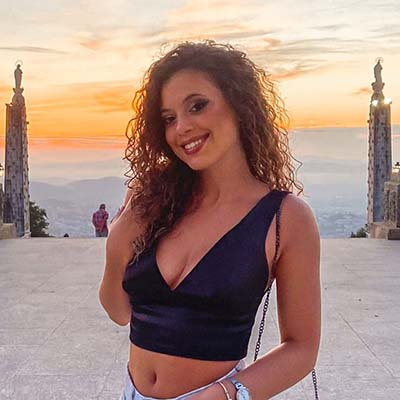
\includegraphics[scale=0.2]{author/mariana.jpg} \\
        62608 - Marco Sousa                           & 93198 - Mariana Marques                       \\
        %\hline                                                                                        \\
        
\includegraphics[scale=0.2]{author/ze.jpg} & 
\includegraphics[scale=0.2]{author/miguel.jpg} \\
        93271 - José Malheiro                         & 94269 - Miguel Fernandes
    \end{tabular}
}

%% Date

\date{\today}

%% Course
\newcommand{\Course}{Licenciatura em Engenharia Informática}

%% Department
\newcommand{\Department}{Escola de Engenharia}

%% UniName
\newcommand{\UniName}{Universidade do Minho}

\newcommand{\UcName}{Sistemas Distribuídos}

\newcommand{\GroupId}{Grupo 12}

%% UniPic
\newcommand{\UniPic}{
\includegraphics[scale=0.09]{uminho.png}}

%% University 
\newcommand{\University}{
    \begin{flushleft}
        \UniPic
    \end{flushleft}
    \textcolor{gray}{\small\textbf{\textsf{\UniName}}}\par
    \textcolor{gray!80!white}{\small{\textsf{\Department}}}\par
    \textcolor{gray!70!white}{\small{\textsf{\Course}}}
}

%% UC
\newcommand{\UC}{
    \begin{flushleft}
        \par\textcolor{titlepagecolor}{  \LARGE\textbf{\textsf{Unidade Curricular de \\ \UcName}}}
    \end{flushleft}
}

%% School Year
\newcommand{\SchoolYear}{
    \small{\textsf{Ano Letivo de 2021/2022}}}


%% Define new command to show title, author and date
\makeatletter
\let\Title\@title
\let\Author\@author
\let\Date\@date
\makeatother

%==========================================================================
% CLASSIFICATION SECTION 
%==========================================================================

%% School Year
\newcommand{\ReceptionDate}{}
%% Responsible
\newcommand{\Responsible}{}
%% Evaluation
\newcommand{\Evaluation}{}
%% Observations
\newcommand{\Observations}{}


%% MAKETEMPLATE
\newcommand{\makecover}{

    %==========================================================================
    % BEGIN COVER PAGE 
    %==========================================================================

    %% Removes page number on footer
    \thispagestyle{empty}

    %% No indentation 
    \setlength{\parindent}{0em}

    %% Put Background defined on \backgroundsetup, in this page
    \BgThispage

    %% Changing geometry to prevent overlay with text
    %% At the end of back cover, geometry is default with \restoregeometry
    \newgeometry{top=3.5cm,left=6cm,right=3cm,bottom=2cm}

    %% builds university info defined previously
    \University
    \vspace{1cm}
    %% builds curricular unity info defined previously
    \UC
    %% builds school year info defined previously
    \SchoolYear

    \vspace*{4cm}
    %% bigger space (i think its the default one) between paragraphs 
    \setlength{\parskip}{1em}

    %% builds title info defined previously
    \par\textbf{\textsf{\huge\Title}}
    \par\textbf{\GroupId}
    \vspace{1cm}
    %% builds author(s) info defined previously
    \par\begin{center}
        \Author
    \end{center}

    \vspace{0.5cm}

    %% builds date info defined previously
    \par\Date
    \restoregeometry
    \pagebreak

    %==========================================================================
    % END COVER PAGE 
    %==========================================================================
}


\graphicspath{ {./assets/} }

\begin{document}

\pagenumbering{gobble}

% builds the cover
\makecover

%==========================================================================
% BEGIN ABSTRACT PAGE
%==========================================================================

%% Abstract name: \Large font size, flushed left and paragraph skip before abstract content

\renewenvironment{abstract}
{\par\noindent\textbf{\Large\abstractname}\par\bigskip}
{}

\begin{flushleft}
    \begin{abstract}
        %=============
        % How to build an abstract
        % https://users.ece.cmu.edu/~koopman/essays/abstract.html
        %=============
        A crescente procura por serviços cliente - servidor, obrigada a que um sistema seja capaz
        de responder a múltiplos pedidos de forma concorrente.
        Como consequência, surge a necessidade de moldar o sistema para que este tenha um comportamento
        determinístico, independentemente da circunstância de utilização.
        Assim, na sequência da Unidade Curricular de \textbf{Sistemas Distribuídos}, surge a oportunidade
        de desenvolver uma aplicação com múltiplos clientes e um servidor, ambos \textit{multi-threaded}.
        
        O projeto proposto corresponde a um sistema de reservas de voos, denominado \textit{Flight Manager}.
        Este, conforme referido, será capaz de ter um servidor que responde a múltiplos clientes, de forma
        concorrente.
        A linguagem de programação utilização foi \textbf{\textit{Java}}, com recurso a \textit{Socket} TCP
        para efetuar a comunicação entre cliente-servidor.
        
        \par \textbf{Área de Aplicação}: Sistemas Distribuídos
        \par \textbf{Palavras-Chave}: Sistemas Distribuídos, \textit{Threads}, \textit{Multithreaded}, 
        \textit{Middleware}, Servidor, Cliente, Serialização, \textit{Data Transfer Object},
        \textit{Sockets}, TCP, \textit{Tagged Connection}
    \end{abstract}
\end{flushleft}

\pagebreak

%==========================================================================
% END ABSTRACT PAGE 
%==========================================================================

%==========================================================================
% BEGIN INTRODUCTION
%==========================================================================

%% Starting page numbering here
\pagenumbering{arabic}

\section{Introdução}

O presente relatório foi escrito no âmbito da Unidade Curricular de Sistemas Distribuídos (SD), sendo o
tendo como principal objetivo apresentar uma possível solução para um Sistema de Gestão de Reservas,
que iremos designar \textit{Flight Manager}, capaz de responder às funcionalidades propostas pela equipa docente.

Assim, será apresentado um sistema \textit{cliente-servidor} que, do lado do servidor,
será capaz de atender múltiplos clientes e, do lado do cliente, será capaz de comunicar com o servidor
e executar métodos assíncronos e síncronos.

Para dar resposta ao proposto, utilizou-se um componente comum a ambos os sistemas, um \textbf{Middleware},
que servirá de ponte de ligação entre os \textit{hosts}.
O objeto de comunicação, será um \textit{Data Transfer Object} e, a partir deste, será derivado
múltiplos objetos relacionados com pedidos e respostas.

Com o desenvolvimento deste projeto, pretende-se apromirar vários conceitos de Sistemas Distribuídos,
tais como:
\begin{itemize}
    \item Programação com \textit{Sockets}
    \item Programação com múltiplas \textit{Threads} (\textit{MultiThread})
    \item Programação Concorrente (estado partilhado)
    \item Exclusão Mútua
    \item Serialização de Objetos
    \item Arquitetura Cliente-Servidor
    \item Desenvolvimento de \textit{Middleware}
\end{itemize}

%==========================================================================
% END INTRODUCTION
%==========================================================================

\section{Análise de Requisitos} \label{chap:analise_requisitos}

O enunciado proposto, remete à conceção e implementação de uma plataforma para gestão de reservas 
de voos, apresentando um conjunto de requisitos funcionais que o sistema deve responder.

A partir do enunciado, identificou-se dois tipos de utilizadores: cliente e adminstrador.
Cada um terá um conjunto de funcionalidades associadas,
tendo sido captadas num Diagrama de Use Case (ver \ref{img:use_case}).

Assim, a nível estrutural, definiu-se três componentes principais:
\begin{itemize}
    \item[\textbf{Cliente}] Interface de interação com o utilizador para utilizar as funcionalidades definidas
    \item[\textbf{Middleware}] Ponte de comunicação entre o cliente e o servidor
    \item[\textbf{Servidor}] Responsável pelo tratamento dos pedidos do cliente
\end{itemize}

Definida a estrutura e as funcionalidades, passou-se para a modelação comportamental do sistema.

\subsection{Modelação Comportamental} \label{strat_esc}

Por forma a permitir uma implementação sustentada, optou-se por efetuar a modelação comportamental 
do sistema.
Para isso, começou-se por definir a forma como o cliente e o servidor iriam comunicar.
Esta revelou-se como uma das etapas fundamentais para o funcionamento da aplicação,
tendo como perspetiva a sua escalabilidade e manutenção.

\subsubsection{Comunicação}

A troca de mensagens entre o cliente e o servidor será mediada por um \textbf{Middleware} (ver \ref{img:middleware}).
Pode-se encontrar um esboço da estratégia analisando o diagrama \ref{img:comunicacao}.

\subsubsection{Middleware}

No \textit{middleware} (ver \ref{img:middleware}), haverá especialização do lado do cliente, por forma a receber respostas e enviar pedidos e
do lado do servidor, para receber pedidos e enviar respostas.
Esta especialização, serve apenas para facilitar a implementação, pois, na realidade, o objeto de comunicação
será sempre o mesmo: uma \mintinline{java}{Frame} que terá no seu corpo informação sobre o pedido, nomeadamente
uma \textit{tag} que a identifica e um \textit{Data Transfer Object} (DTO).
Este último, será um dos principais atores na troca de informação, pois a partir da sua especialização,
será possível criar cada um dos pedidos e cada uma das respostas, conforme o conteúdo necessário.
Com o objetivo de generalização do código, colocou-se que a classe \textit{DTO} será abstrata e terá como método,
também este abstrato, a serialização (\textit{serialize}).

\subsubsection{Servidor}
Dotado de um \textit{ServerSocket}, este será capaz de estabelecer ligação com cada cliente,
sendo-lhe atribuída uma \textit{Thread} e \textit{Socket} própria, partilhando um estado comum com arquitetura \textbf{Facade}: 
\mintinline{java}{IFlightManager} (ver \ref{img:flight_manager}).
Neste, poderá identificar-se dois subsistemas: \textit{Booking Manager} e \textit{User Manager}.

Sendo um servidor \textit{multi-threaded}, é necessário que haja controlo de concorrência.
Assim, pode-se verificar junto dos diagramas que serão referenciados e na secção de implementação
as estratégias utilizadas.

Utilizou-se os princípios \textit{SOLID} \cite{wiki:solid} ao longo da implementação de todo o código,
assim como o seu planeamento.

\subsubsection{Booking Manager}

Lógica relacionada com os processos de reserva de vôos, tais como os vôos diários disponíveis
no sistema, uma abstração do dia (com os respetivos vôos associados) e as reservas propriamente ditas.
Ver \ref{img:booking_manager}

\subsubsection{User Manager}
Lógica relacionada com a gestão dos utilizados. Tal como referido, existe dois tipos:
\textit{Administrador} e \textit{Cliente}.
Para permitir a escalabilidade do sistema, ambos especializam uma classe abstrata designada
\textbf{Utilizador}. Ver \ref{img:user_manager}

\subsubsection{Flight Manager}
Conforme referido, foi utilizada uma estratégia \textit{Facade} para o desenvolvimento
do estado partilhado no \textbf{Servidor}.
Assim, a classe agregadora designa-se \textit{FlightMinegerFacade} que implementa a API definida
pela interface \textit{IFlightManager}.
Como é habitual neste tipo de estratégias, esta classe permite conjugar métodos relacionados com 
o \textit{Booking Manager} e o \textit{User Manager}.

\subsubsection{Cliente}
Em termos estruturais, o cliente apresenta uma lógica bastante mais simples.
No entanto, por forma a implementar algumas funcionalidades adicionais, nomeadamente
a possibilidade de efetuar uma reserva sem que se tenha de esperar pela sua conclusão,
houve necessidade de implementar um \textit{ClientManager} (\ref{sec:client_manager}).

\subsubsection{ClientManager} \label{sec:client_manager}
Classe que permite ao cliente que este seja \textit{multi-threaded} mas apenas ao nível dos pedidos,
com o objetivo de serem não bloqueantes.
Quer isto dizer que, apesar de haver uma \textit{thread} principal a tratar do interface
e da lógica do cliente, este pode utilizar métodos assincronos, que são executados por 
outras \textit{threads} que lhe ficam associadas.

\section{Implementação}
Devido ao curto número de páginas definido pela equipa docente, será apenas abordado alguns pontos
considerados fulcrais na implementação do sistema proposto.

\begin{multicols}{2}[\section{Middleware}]
    Tanto o cliente como o servidor utilizam a mesma classe base para 
    gerir a ligação, \textit{TaggedConnection}.
    Cada mensagem foi encapsulada numa \textit{Frame}
    que é identificada por uma \textit{tag}.
    Tem, ainda, o nome da classe que está a transportar e
    a própria classe.
    Desta forma, permite-te que se faça a \textit{deserialization}
    de forma bastante simples e elegante.
    Para isso, foi introduzido um \mintinline{java}{Map<String, Class<? extends DTO>>}
    que mapeia o nome da classe para o seu tipo concreto com entradas do tipo
    \mintinline{java}{entry(UnitDTO.class.getSimpleName(), UnitDTO.class)}.
    Depois desta etapa, obtém-se o método \textit{deserialize} da classe que,
    conforme definido, é implementado por todas as 
    \mintinline{java}{Class<? extends DTO>}.
    Assim, a leitura do \textit{Socket} é efetuada em 3 etapas:
    \begin{enumerate}
        \item Ler o nome da classe
        \item Mapear o nome para o tipo concreto
        \item Invocar p método \textit{deserialize} adequado
    \end{enumerate}
    \begin{minted}{java}
            Class<? extends DTO> p = getMapping(cName);
            Method m = p.getMethod("deserialize", DataInputStream.class);
            DTO dto = (DTO) m.invoke(null, in);
            return new Frame(tag, dto);
    \end{minted}
    Por forma a melhorar a eficiência do cliente, foi desenvolvido
    um \textit{Demultiplexer} que corresponde a ter uma \textit{Thread}
    em execução apenas para efetuar a leitura da \textit{Socket}, 
    efetuar o \textit{deserialize} adequado e adicionar à \textit{Entry}
    correpondente, identificada pela \textbf{tag}.
    Posteriormente, a \textit{Thread} que estava à espera é notificada para
    que possa ler a partir da \textit{Queue} de \textbf{DTO} associado.
    \begin{minted}{java}
        final Condition cond = mLock.newCondition();
        final ArrayDeque<DTO> queue = new ArrayDeque<>();
        int waiters = 0;
    \end{minted}
    
    Ainda a este nível, foi implementado uma classe que especializa a \textit{Thread}:
    \mintinline{java}{class QueryThread}.
    Pretende-se que esta permita uma chamada assíncrona do método.
    Para isso, o construtor recebe um \textbf{DTO} (\textit{Query}), a \textit{tag}
    e um apontador para o \textit{Demultiplexer}: 
    \mintinline{java}{QueryThread(DTO queryDTO, int tag, Demultiplexer c)}.
    Ao utilizar esta classe, permite que um pedido ao servidor seja feito
    por uma \textit{Thread} especifica para o efeito.
    Caso pretenda esperar pelo resultado, utilizará o método \mintinline{java}{public DTO result()}.
    Se pretender obter o resultado (caso já esteja disponível), utilizará o método
    \mintinline{java}{public DTO getResponse()}.
    Com esta estratégia, foi possível implementar a funcionalidade adicional proposta
    que corresponde ao paralelismo na execução de pedidos, de uma forma generalizada e escalável.    
    
\end{multicols}

\begin{multicols}{2}[\section{Cliente}] \label{sec:cliente}
    Posto a implementação definida no ponto anterior, procedeu-se à implementação
    do \textit{interface} gráfico de interação com o utilizador.
    Atendendo que este não era o foco do projeto, implementou-se uma versão estritamente
    essencial.
    Assim, pode-se encontrar um sistema de menus que foi representado numa máquina
    de estados (ver \ref{img:menu_estados}).
    
    Para lidar com os pedidos, introduziu-se dois métodos principais: (i) \mintinline{java}{public QueryThread asyncHandler(DTO dto)}
    e (ii) \mintinline{java}{public DTO queryHandler(DTO dto)}.
    \begin{itemize}
        \item[(i)]{
              Coloca uma nova \textit{thread} em execução, ficando esta a aguardar pela resposta.
              Adiciona-a, ainda, ao \textbf{ClientManager} (\ref{sec:client_manager}) para ficar acessível
              ao cliente.
              }
        \item[(ii)]{
              Utiliza o método (i) e fica a aguardar pelo resultado através do método
              \textit{result()} que efetua uma espera passiva pela conclusão da \textit{thread}.
              Corresponde à transformação de um método assincrono em um síncrono.
              }
    \end{itemize}
    Para além destes, existe ainda um método específico para lidar com o login,
    pois tem a particularidade de definir no cliente o \textbf{token} que recebeu
    do servidor e terá de utilizar nas comunicações futuras.
    
    A estratégia utilizada para pedir algo ao servidor corresponde, portanto, à 
    sequência de 3 etapas:
    \begin{enumerate}
        \item {
              Construção do \textit{DTO} associado ao pedido, pedindo ao cliente os parâmetros
              necessários através do \textit{Stdin};
              } 
        \item {
              Utilização do método síncrono ou assíncrono (queryHandler ou asyncHandler).
              }
        \item {
              Leitura e apresentação da resposta do servidor, em conformidade
              com o recebido
              }
    \end{enumerate}
    Como exemplo, pode-se verificar o menu \textbf{reserva} em que é efetuado um
    pedido de forma assincrona (apenas a componente de pedir a query):
    \begin{minted}{java}
        BookFlightQueryDTO q = new BookFlightQueryDTO(params, min, max);
        this.c.asyncHandler(q);
        System.out.println("O seu pedido foi efetuado.");
        System.out.println("Pode acompanhar no menu de pendentes!");
    \end{minted}
    Neste excerto de código, pode-se verificar que não é esperado a resposta do 
    pedido efetuado. 
    O sistema remete o cliente para um menu próprio onde pode consultar
    pedidos (de reservas) que estejam concluídos.
\end{multicols}

\begin{multicols}{2}[\section{Servidor}]
    Por ser um servidor \textit{multi-threaded}, a sua implementação foi
    mais complexa, por forma a evitar \textit{dead-locks}, alteração de estado
    a meio de transações, entre outros.
    Assim, houve a necessidade de implementar vários \textit{Locks} em níveis
    diferentes da estrutura e para controlo de diferentes estados.
    
    Portanto, o servidor segue a seguinte sequência de acontecimentos:
    \begin{enumerate}
        \item Efetua a leitura do estado (FlightMinegerFacade) a partir de um ficheiro de objetos;
        \item Inicia um \textit{Logger}
        \item Injeta esse estado numa classe que estará à escuta de uma \textit{ServerSocket} na porta $4444$;
        \item Inicia a \textit{thread} paralela
        \item Coloca a \textit{thread} principal à escuta do \textit{System.in}
    \end{enumerate}
    Começando pelo último ponto, é permitido que o utilizador termine o servidor a qualquer
    altura. Esta terminação é efetuada de forma eloquente, i.e. começa por fechar a socket
    de entrada no servidor (não aceitando novas ligações), mas permite que os clientes ligados terminem as suas transações.
    Apenas quando todos os clientes fecharem a conexão, o servidor encerrará e gravará 
    o seu estado atual num ficheiro de objetos.
    
    Sempre que um cliente se estabelece ligação com um servidor, é criado uma
    nova \textit{thread} designada \mintinline{java}{class ServerWorker}
    que terá acesso ao modelo (estado partilhado), à sua \textit{Socket}
    e a uma \mintinline{java}{class ThreadHandler} (partilhada).
    
    Começando pela \textit{ThreadHandler}, permite a gestão dos clientes que estão
    ligados ao servidor.
    O método \textit{run()} está em espera passiva e sempre que há uma nova ligação,
    percorre a sua lista de \textit{threads} e remove as que já não estiverem ativas.
    Esta classe é utilizada, também, quando se pretende encerrar o servidor, pois será
    esta que ficará à espera que todos os clientes terminem a sua transação.
    
    O \textit{ServerWorker} permite que cada \textit{thread} que estabeleceu ligação
    lide com os pedidos do cliente.
    Tal como anteriormente, utilizou-se uma estratégia semelhante para lidar com a conversão
    do \textbf{DTO} abstrato para o especifico enviado pelo cliente.
    Utiliza-se um \mintinline{java}{Map<String, Function<QueryDTO, DTO>>} que permite,
    a partir do nome da classe, chamar o método que efetuará o tratamento do pedido.
    As entradas do mapa são do tipo:
    \begin{minted}{java}
        entry(LoginQueryDTO.class.getSimpleName(), (x) -> this.loginHandler(x))
    \end{minted}
    Desta forma, sempre que o servidor recebe um pedido, para além de escrever um
    \textit{Log} que permite ter um histórico de pedidos recebidos, é capaz de o converter
    num resultado e responder ao cliente aplicando o método obtido no mapeamento:
    \begin{minted}{java}
	public void requestHandler(Frame f)  {
		QueryDTO dto = (QueryDTO) f.getDto();
		String method = dto.getClass().getSimpleName();
		DTO r = getMapping(method).apply(dto);
		this.c.send(new Frame(f.tag, r));
	}
    \end{minted}
    Cada um dos métodos utiliza a API definida como \textit{IFlightManager}
    que é implementada pela \mintinline{java}{class FlightManagerFacade}.
    Consequentemente ao servidor aceitar pedidos de múltiplos clientes em simultâneo,
    i.e. haverá concorrência no acesso aos recursos disponibilizados
    Portanto, houve a necessidade de definir variáveis com acesso crítico, assim
    como regiões críticas.
    Para acesso a estas regiões, utilizou-se a classe \textit{ReentrantLock} garantindo
    o acesso \textit{single-threaded}.
    Ao implementar a lógica relacionada com a gestão de reservas e utilizadores,
    identificou-se dois padrões: lógica relacionada apenas com um dos sub-sistemas
    (\textbf{Utilizadores} ou \textbf{Reservas}) e lógica relacionada com métodos
    que têm dependencias em ambos.
    
    Em ambas as situações, procurou-se utilizar os \textbf{locks} de nível superior
    durante o menor tempo possível.
    Assim, começa-se por obter o \textbf{lock} para variáveis gerais e, posteriormente,
    obtém-se o \textbf{lock} da classe específica, procedendo à libertação do \textbf{lock}
    anteriormente adquirido.
    Um exemplo da estratégia utilizada:
    \begin{minted}{java}
		this.l.lock();
		BookingDay bd;
		try {
			bd = this.getBookingDay(LocalDate.now());
			bd.l.lock();
		} finally {
			this.l.unlock();
		}
		try {
			bd.closeDay();
			return true;
		} finally {
			bd.l.unlock();
		}
    \end{minted}
    No caso de soluções que dependam de ambos os sub-sistemas, houve necessidade
    de ser o \textit{Facade} a obter o \textbf{lock} da estrutura de um sistema e,
    posteriormente, executar o método pretendido no outro sistema.
    No final, liberta o \textbf{lock} adquirido.
    Um exemplo de métodos que dependem de ambos os sistemas:
    \begin{minted}{java}
		if (users.hasUser(user)) {
			User u = users.getUser(user);
			u.lock.lock();
			String bookId;
			try {
				bookId = booking.bookFlight(user, percurso, de, ate);
				users.addReserva(user, bookId);
			} finally {
				u.lock.unlock();
			}
			return bookId;
		}
		throw new UserNaoExistente(user);
    \end{minted}
\end{multicols}

\begin{multicols}{2}[\section{Funcionalidade Adicional}]
    Introduziu-se a estratégia de travessia de grafos, permitindo
    a construção de caminhos entre dois destinos.
    Neste caso, o caminho foi limitado (conforme indicado no enunciado)
    a um máximo de 2 paragens, correspondendo a 4 cidades (A\rightarrow B
    \rightarrow C \rightarrow D).
    A estrutura de suporte ao grafo é \mintinline{java}{Map<String, List<String>>}
    que permite, para uma dada origem, saber a lista de destinos possíveis.
    
    Sempre que é adicionado um novo destino (vôo), este é adicionado ao grafo.
    Para garantir o acesso concorrente ao grafo, sem afetar a eficiência do servidor,
    optou-se por lhe alocar um \textbf{lock} específico.
    \vspace{1cm}
    \begin{minted}{java}
			g.lock();
			try {
				if (grafo.containsKey(v.getOrigem())) {
					List<String> arestas = grafo.get(v.getOrigem());
					arestas.add(v.getDestino());
					grafo.put(v.getOrigem(), arestas);
				} else {
					List<String> arestas = new ArrayList<>();
					arestas.add(v.getDestino());
					grafo.put(v.getOrigem(), arestas);
				}
			} finally {
				g.unlock();
			}
    \end{minted}

    Por último, conforme já abordado no Cliente (ver \ref{sec:cliente}), implementou-se
    a possibilidade deste realizar pedidos que fiquem em execução em segundo plano,
    podendo, desta forma, continuar a trabalhar na aplicação sem esperar pela
    sua conclusão.
\end{multicols}

\section{Considerações Finais}
\subsection{Conclusões}
Com o objetivo de facilitar a implementação do sistema, começou por se efetuar a modelação
funcional, estrutural e comportamental com recurso à ferramenta \textit{Visual Paradigm}.
Ao utilizar esta estratégia, permitiu ter uma visão mais abstrata do problema, levando
a uma solução mais estruturada, escalável e sustentável.

Uma das principais dificuldades durante a implementação da solução, deveu-se à decisão de quando 
e como utilizar os \textit{locks}.
Para tal, conforme referido, começou por se identificar regiões críticas e fez-se
um processo de implementação iterativa, i.e. começou por se introduzir \textit{locks}
ao nível da raíz e procedendo à sua especialização.

Não obstante, a dificuldade indicada, procurou-se que a implementação fosse o mais simples
e generalizável possível. Para isso, procedeu-se à introdução de um Middleware cujo objeto
de comunicação fosse facilmente identificável. Este requisito levou à introdução de uma 
\textit{Frame} que encapsula um \textbf{DTO}, podendo ser especializado como uma \textit{query} ou uma resposta.

Ao nível de controlo de concorrência, pode-se acrescentar que se procurou obedecer
às regras lecionadas ao longo da UC de Sistemas Distribuídos, nomeadamente
através da aquisição de \textit{lock} de forma ordenada, assim como a respetiva
libertação. Esta estratégia foi implementada quando se precisava de adquirir controlo
sobre várias estruturas em simultâneo.

\subsection{Trabalho Futuro}

Com a perspetiva de melhorar a interação com o cliente, seria uma mais valia fazer
uma restruturação do \textit{User Interface}.
Especificamente, através de uma \textit{interface} mais atrativa e utilizável.
Mediante a nova UI, seria possível que os pedidos que fossem efetuados de forma assincrona,
apresentassem o seu resultado com uma \textit{pop-up} ou algum tipo de aviso que não interfira
diretamente com o que o cliente se encontra a fazer. Por exemplo, no sistema desenvolvido,
caso os pedidos assincronos fossem apresentados mal terminassem, podiam intercalar
com um \textit{output} que estive a ser exibido.

Poderia, ainda, introduzir-se persistência através de utilização de \textbf{Bases de Dados}.
Tal funcionalidade não foi implementada, pelo facto dos elementos do grupo não terem conhecimentos
sobre esse tipo de sistemas.

Para além destes, será necessário desenvolver mais testes para validar o funcionamento da aplicação.

O aperfeiçoamento da aplicação, de modo a chegar a um estado competitivo para o mercado atual, passaria pela
implementação de várias e diferentes funcionalidades que lhe permitisse ser distinguido dos restantes concorrentes.

\printbibliography
%==========================================================================
% BEGIN LISTA DE SIGLAS E ACRÓNIMOS
%==========================================================================

%% Portuguese babel does not translate this environment
\renewcommand{\nomname}{Lista de Siglas e Acrónimos}

%% Text that can be shown before acronyms list
\renewcommand{\nompreamble}{}

%% acronyms
\nomenclature[01]{\textbf{SD}}{Sistemas Distribuídos}
\nomenclature[02]{\textbf{DTO}}{\textit{Data Transfer Object}}
\nomenclature[03]{\textbf{UC}}{Unidade Curricular}
\nomenclature[04]{\textbf{plataforma}}{Sistema de gestão de reservas de voos}
\nomenclature[05]{\textbf{sistema}}{Sistema de gestão de reservas de voos}
\nomenclature[06]{\textbf{aplicação}}{Sistema de gestão de reservas de voos}
\nomenclature[06]{\textbf{programa}}{Sistema de gestão de reservas de voos}

%% Show acronyms
\printnomenclature

%==========================================================================
% END LISTA DE SIGLAS E ACRÓNIMOS
%==========================================================================

%==========================================================================
% BEGIN ANEXOS
%==========================================================================

\section{Anexos}
\subsection{Anexo 1 - Diagrama de Use Case}
\begin{figure}[!ht]
    \centering
    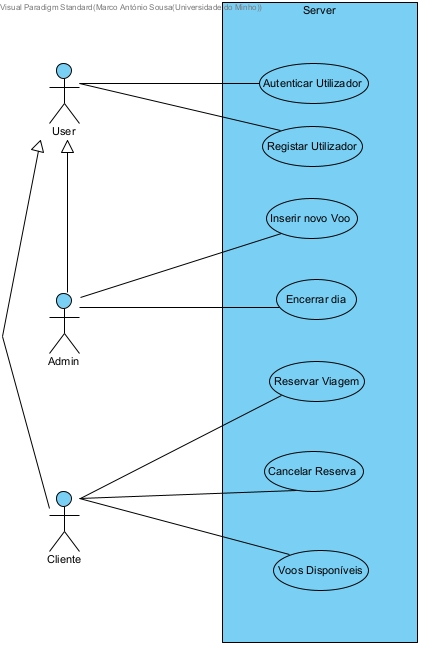
\includegraphics[scale=0.75]{diagramas/useCaseDiagram.jpg}
    \caption{Diagrama de Use Case} \label{img:use_case}
\end{figure}

\begin{landscape}
    \subsection{Anexo 2 - Diagrama de Comunicação}
    \begin{figure}[!ht]
        \centering
        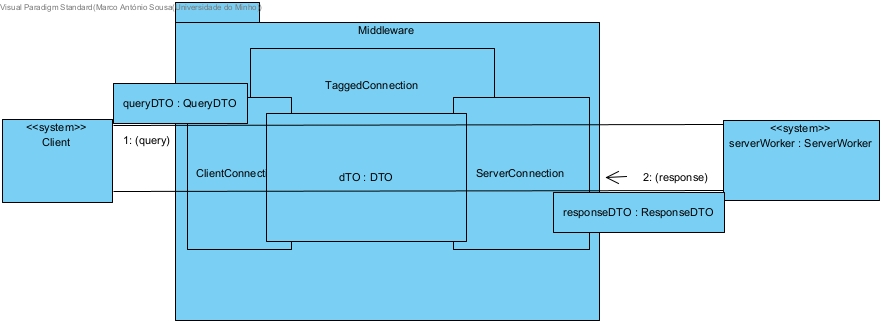
\includegraphics[width=\linewidth]{diagramas/MiddlewareCommunicationDiagram.jpg}
        \caption{Diagrama de Comunicação - versão $\beta$} \label{img:comunicacao}
    \end{figure}
\end{landscape}

\begin{landscape}
    \subsection{Anexo 3 - Diagrama de Classes do Middleware}
    \begin{figure}[!ht]
        \centering
        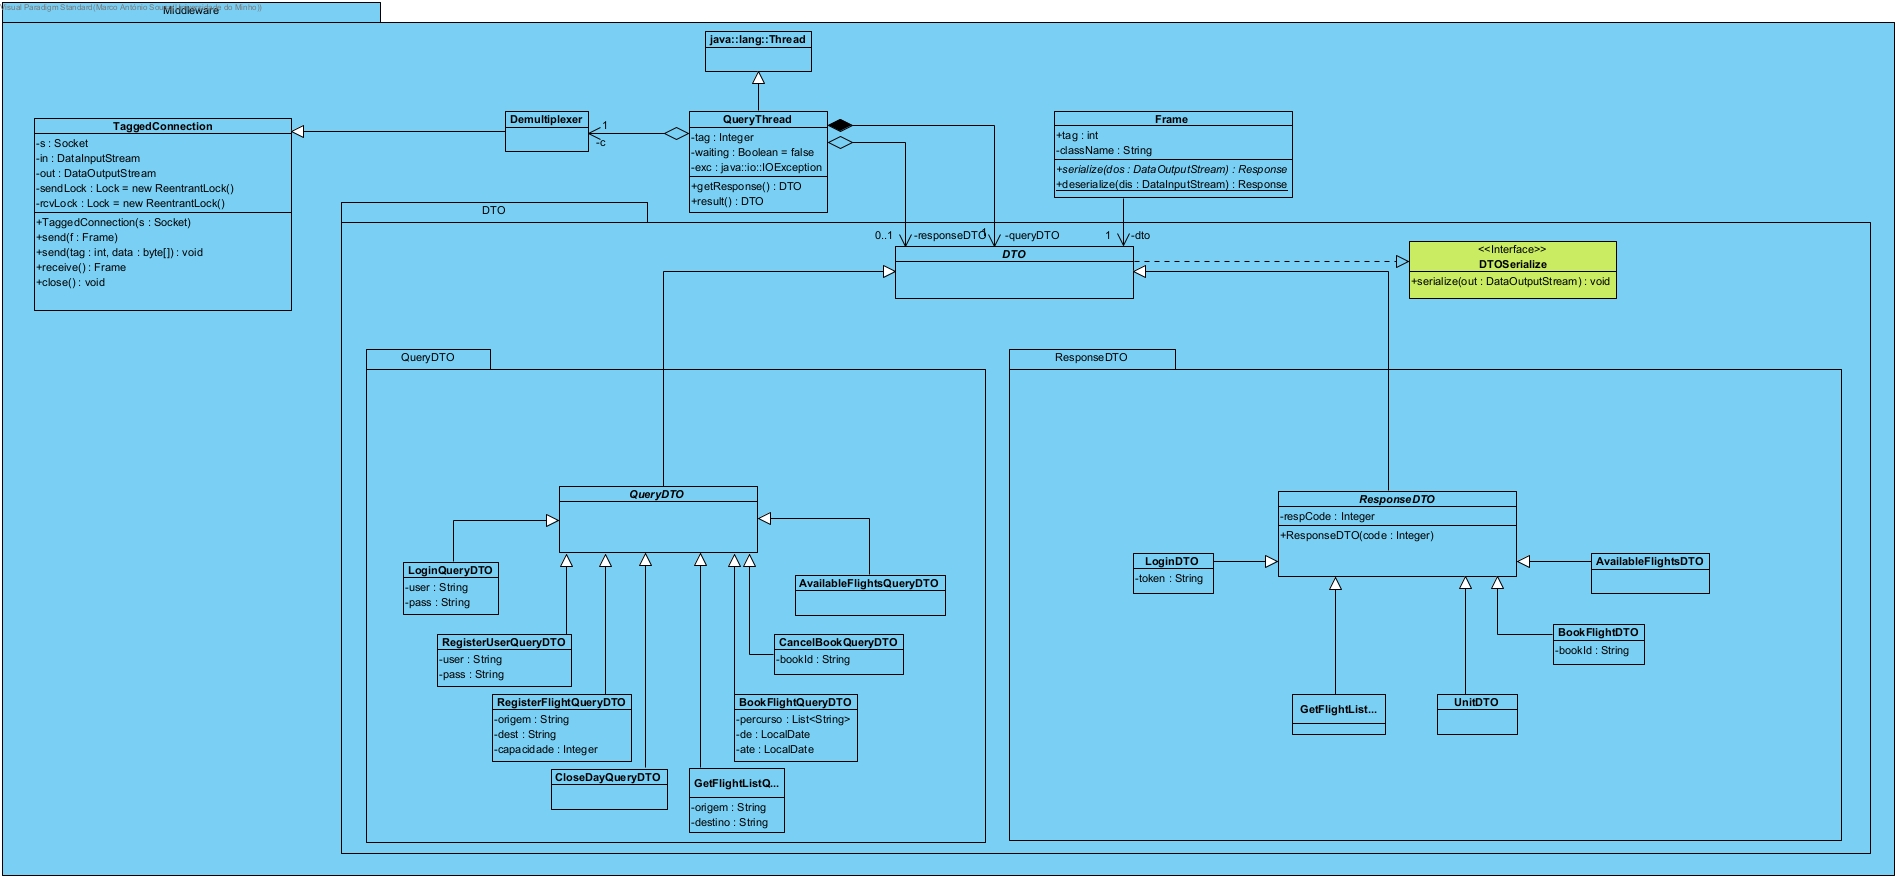
\includegraphics[width=\linewidth]{diagramas/MiddlewareClassDiagram.jpg}
        \caption{Diagrama de Classes - Middleware} \label{img:middleware}
    \end{figure}
\end{landscape}

\begin{landscape}
    \subsection{Anexo 4 - Diagrama de Classes do FlightManager (Servidor)}
    \begin{figure}[!ht]
        \centering
        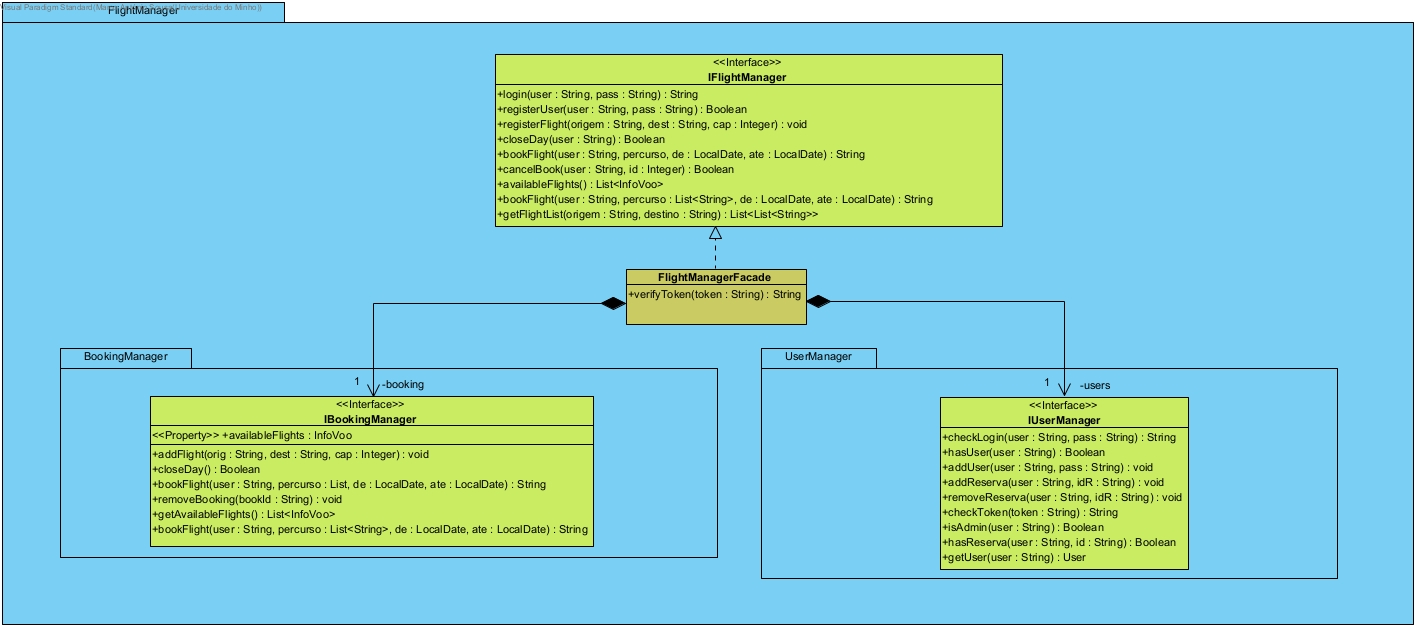
\includegraphics[width=\linewidth]{diagramas/FlightManager.jpg}
        \caption{Diagrama de Classes - FlightManager} \label{img:flight_manager}
    \end{figure}
\end{landscape}

\begin{landscape}
    \subsection{Anexo 5 - Diagrama de Classes do Booking Manager (Servidor)}
    \begin{figure}[!ht]
        \centering
        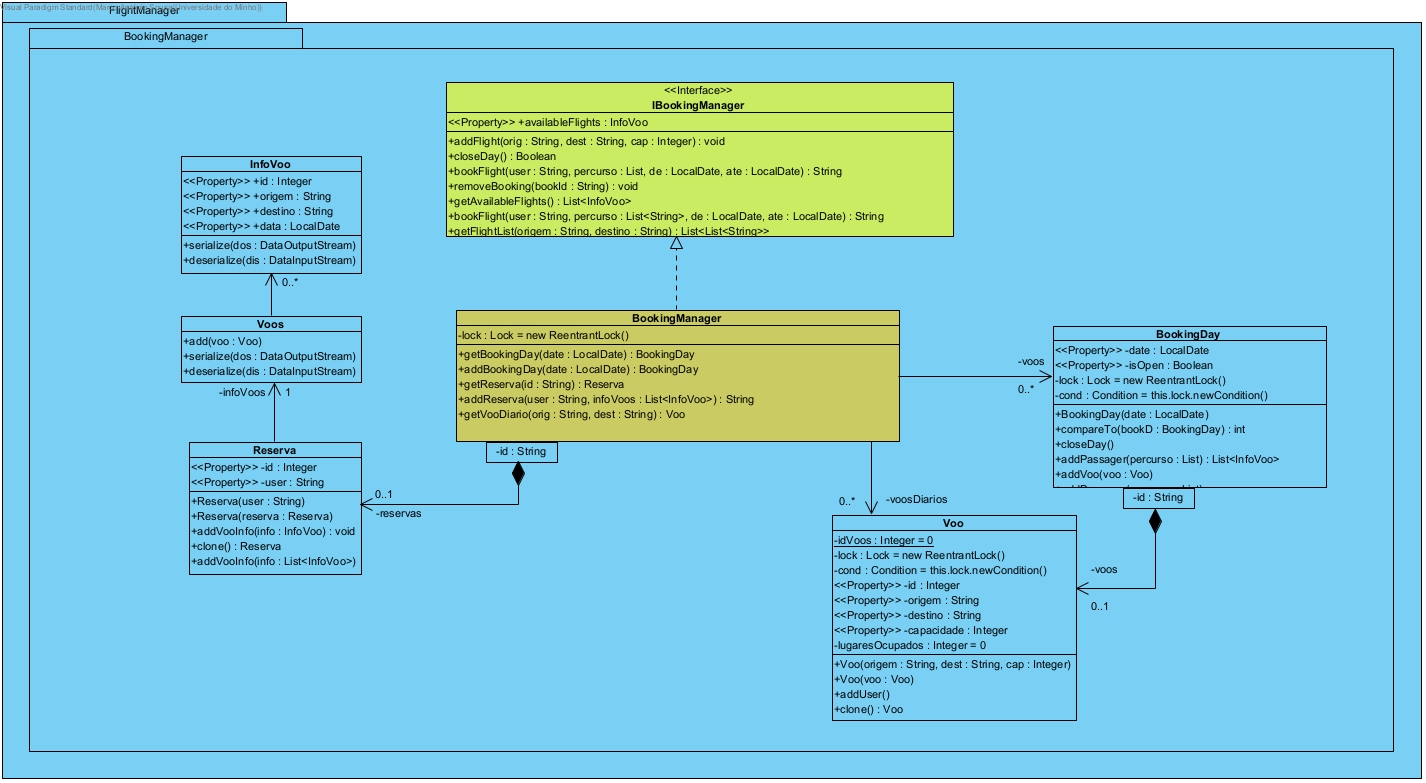
\includegraphics[width=0.9\linewidth]{diagramas/BookingManagerClassDiagram.jpg}
        \caption{Diagrama de Classes - BookingManager} \label{img:booking_manager}
    \end{figure}
\end{landscape}

\begin{landscape}
    \subsection{Anexo 6 - Diagrama de Classes do User Manager (Servidor)}
    \begin{figure}[!ht]
        \centering
        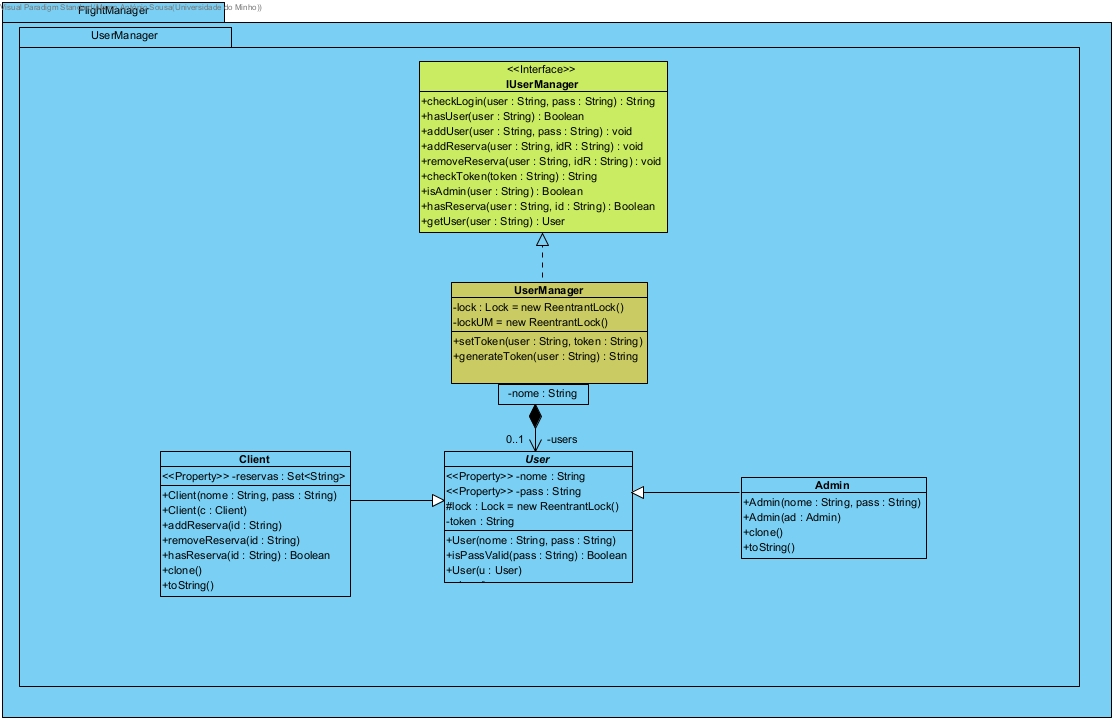
\includegraphics[width=0.75\linewidth]{diagramas/UserManagerClassDiagram.jpg}
        \caption{Diagrama de Classes - BookingManager} \label{img:user_manager}
    \end{figure}
\end{landscape}

\begin{landscape}
    \subsection{Anexo 7 - Diagrama Pseudo-Estado Menu de UI}
    \begin{figure}[!ht]
        \centering
        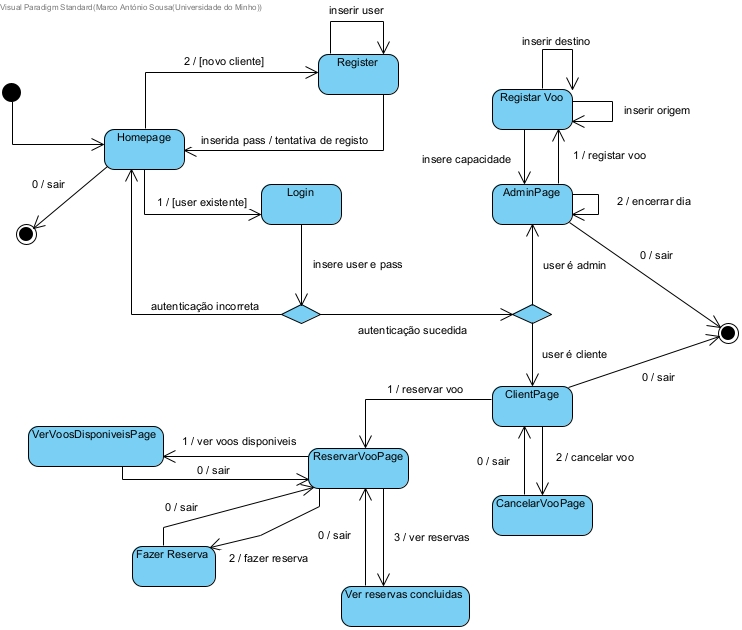
\includegraphics[scale=0.7]{diagramas/MenuUI.jpg}
        \caption{Diagrama de Estado - Sistema de Menu} \label{img:menu_estados}
    \end{figure}
\end{landscape}

%==========================================================================
% END ANEXOS
%==========================================================================

\end{document}